% latex article template

% cheat sheet(eng): http://www.pvv.ntnu.no/~walle/latex/dokumentasjon/latexsheet.pdf
% cheat sheet2(eng): http://www.pvv.ntnu.no/~walle/latex/dokumentasjon/LaTeX-cheat-sheet.pdf
% reference manual(eng): http://ctan.uib.no/info/latex2e-help-texinfo/latex2e.html

% The document class defines the type of document. Presentation, article, letter, etc. 
\documentclass[12pt, a4paper]{article}

% packages to be used. needed to use images and such things. 
\usepackage[pdfborder=0 0 0]{hyperref}
\usepackage[utf8]{inputenc}
\usepackage[english]{babel}
\usepackage{graphicx}
\PassOptionsToPackage{hyphens}{url}

% hides the section numbering. 
\setcounter{secnumdepth}{-1}

% Graphics/image lications and extensions. 
\DeclareGraphicsExtensions{.pdf, .png, .jpg, .jpeg}
\graphicspath{{./images/}}

\title{
	Project Implementation \\
    TDT4240 - Group A14 \\
	\\
}
\author{
	\underline{Group members:} \\
    Bremnes, Jan A. S.\\
    Johanessen, Stig Tore\\
	Hesselberg, Håkon \\
    Kirø, Magnus L.\\
	Randby, Simon \\
    Tørresen, Håvard\\
}

\date{\today}

\begin{document}
\maketitle
\paragraph{Chosen COTS:} Andoid
\paragraph{Primary quality attribute:} Modifiability
\paragraph{Secondary quality attribute:} Testability \\

\pagenumbering{arabic}

\begin{abstract}
This is the paper's abstract \ldots
\end{abstract}

\newpage
\tableofcontents
\newpage

\section{Introduction}

\subsection{Description of the project and the phase (implementation and
testing)}

The point of this entire project is to create a game for Android. Our game
concept is based on the classic game Battleship. We have recreated it and made
room for improvements and further expansion of the game concept. 

This phase of the project has been about the implementation and testing of the
game.

What we’ve created is a version with basic functionality, with focus on
architecture, modularity and expandability. The architecture of the game is such
that it should be possible to add additional functionality while keeping the
core structure, while keeping it easy to maintain.

\subsection{Description of game concept}
You are given a fleet of ships to arrange on a grid either horizontally or
vertically. After placing the ships the game proceeds in a series of rounds.
Taking alternating turns, each player fire at their opponent’s grid, attempting
to guess where the enemy ships are. You will see if you hit or miss an enemy
ship, and you use this information to get a picture of your opponent’s fleet.
When a player has successfully eliminated all opposing ships, the game is over
and that player wins.

\subsection{Structure of the document}
This document contains the relevant information to the implementation and
testing we’ve done. To begin with is this introduction, followed by a user’s
manual describing how to install and play the game. After that comes the design
and implementation details, then the test reports. Lastly there will be a
description of the inconsistencies between architecture and implementation, in
addition to a listing of the problems and issues we ran into.

\section{User Manual}
\subsection{Installation}
Description of how to install, compile and run the game/robot.
TODO 

\subsection{Tutorial}
Sound can be disabled at any time by clicking on menu, then disabling from
settings.
TODO write a little description useing refs to images. 

% starticon
\begin{figure}[h!]
    \centering
    
\includegraphics[width=.4\textwidth]{starticon} 
    \caption{Launch the application by clicking on the icon}
    \label{fig:starticon}
\end{figure}

% newgame
\begin{figure}[h!]
    \centering
    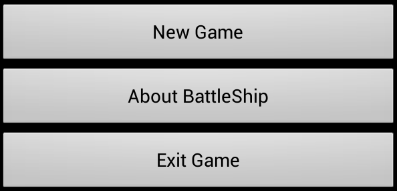
\includegraphics[width=.6\textwidth]{newgame} 
    \caption{Start a new game by clicking "new game"}
    \label{fig:newgame}
\end{figure}

% choseboardsize
\begin{figure}[h!]
    \centering
    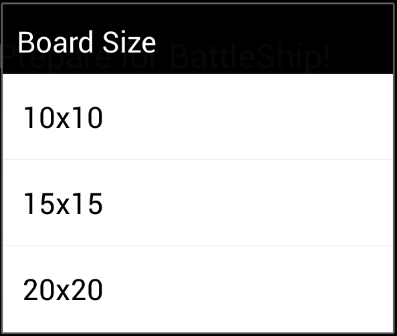
\includegraphics[width=.4\textwidth]{choseboardsize}
    \caption{Chose 10x10 as a board size}
    \label{fig:choseboardsize}
\end{figure}

% placeships
\begin{figure}[h!]
    \centering
    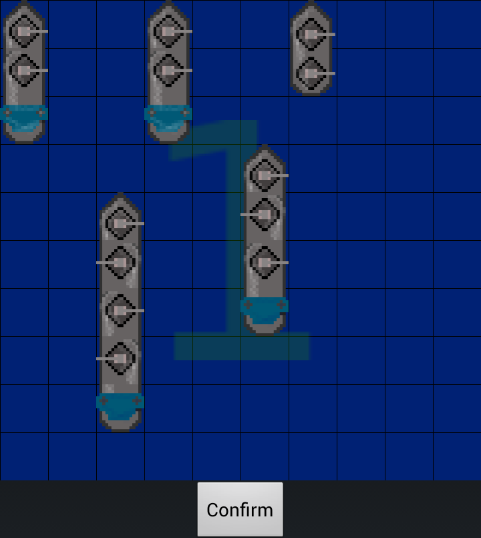
\includegraphics[width=.4\textwidth]{placeships}
    \caption{Drag and drop ships to place them where you want, then click
confirm. Ships can’t be placed on top of eachother}
    \label{fig:placeships}
\end{figure}

% flipships
\begin{figure}[h!]
    \centering
    
\includegraphics[width=.4\textwidth]{flipships}
    \caption{Double-click a ship to flip it.}
    \label{fig:flipships}
\end{figure}

% confirmplacement
\begin{figure}[h!]
    \centering
    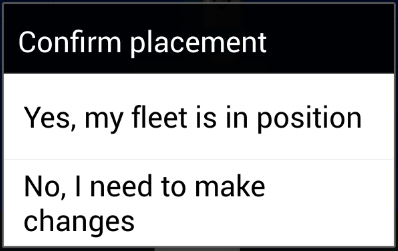
\includegraphics[width=.4\textwidth]{confirmplacement}
    \caption{When you are sure your fleet is correctly placed, click "Yes, my
fleet is in position". Repeat steps for player 2}
    \label{fig:confirmplacement}
\end{figure}

% fire
\begin{figure}[h!]
    \centering
    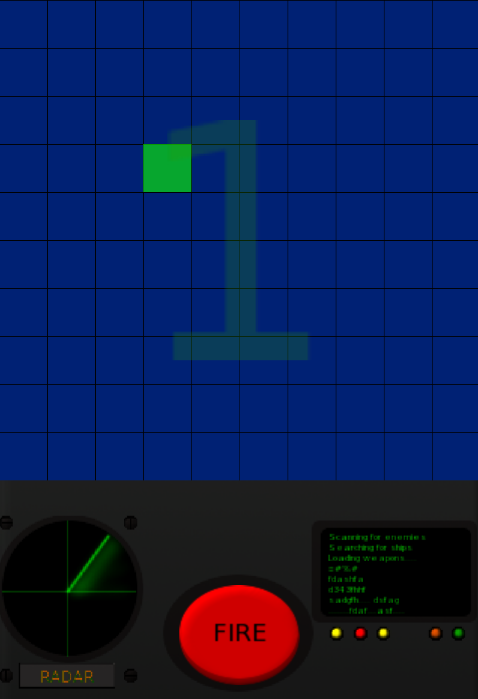
\includegraphics[width=.4\textwidth]{fire}
    \caption{Select a location you wish to fire, it will show up in green. Click
fire.}
    \label{fig:fire}
\end{figure}

% impact
\begin{figure}[h!]
    \centering
    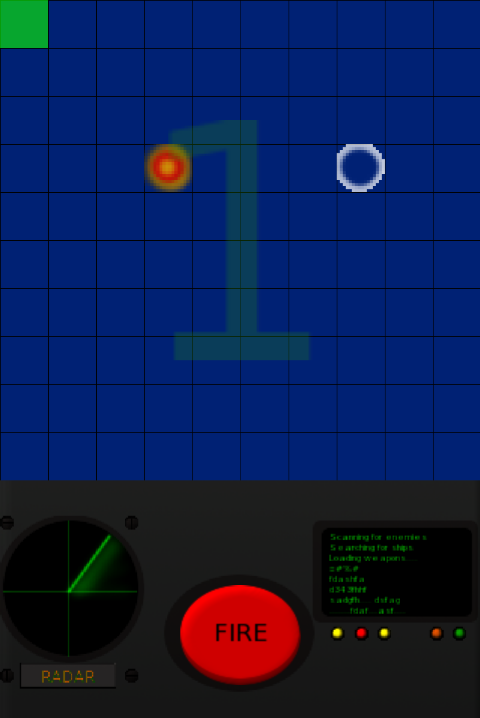
\includegraphics[width=.4\textwidth]{impact}
    \caption{A hit will show up as a red circle (left). As miss shows up as a
white ring (right). Keep firing until either player 1 or 2 has won.}
    \label{fig:impact}
\end{figure}


\section{Design/Implementation details}
More detailed description of how the game/robot controller was designed and
implemented, including complete class-diagram, description of the implemented
classes etc.

\subsection{Detailed description of design process}
TODO !!
\subsection{How it was implemented}

Our implementation deviated from our architecture plans in two areas: the use of
MVC, and abstract factories. Additionally, there were several features that we
did not have time to implement.

While figuring out how to do various things in android, we discovered that the
platform is actually not designed for MVC, probably due to fears of overloading
the weak hardware on the first devices that were available. Due to this, android
uses a blend of java and XML to define global constants and graphical
components, making it hard to stick to traditional java conventions on message
passing and creating objects. The result is that we are not using a strict MVC
design, but utilize some minor "hacks" to get things to do what we want.

Our plans show a myriad of factories to create various kinds of platforms and
devices. During implementation, we realized it would be simpler to make a
general type of each, and instead allow them to be configured via a
settings-file. The idea would be that the factory gets a configuration, and then
produces a set of items according to those specifications.

As for the missing features, this is a result of lacking experience with android
development, and poor planning of working hours, resulting in several long
nights during the last week. The things we did not implement are as follows:

\begin{itemize}
	\item Devices: 
		\subitem We decided this was not a high priority feature, and so it is
not possible to equip the platforms with various deices that affect how many, and what kind of
shots the player can fire upon his opponent.
	\item Settings:
		\subitem We currently only have settings for toggling sound effects on and off
	\item Networking: 
		\subitem This was a very low priority feature that would only be implemented if all other
things were in place.
\end{itemize}

\subsection{Class diagram}

\paragraph{About} \\
	The dialogbox that pops up when clicking the "About" button in the main menu.

\paragraph{BattleShip} \\
	The main screen. Diplays the main menu, and let's users start a new game, view the about screen or exit the game. Contains methods for displaying a Settings-menu when the user clicks the Menu button.
When user chooses to start a new game, a GameActivity is started.

\paragraph{Prefs} \\
	The settings menu, allows the user to set preferences. Contains only the possiblity for turning sound effects on or off, but other choices can easily be added

\paragraph{GameActivity} \\
	This class creates the screen layout, and holds an instance of the GameViewer and GameController classes. A settings menu is also enabled here. Creates the SoundPool which contains the sound effects.

\paragraph{GameViewer} \\
	Draws the battlefield.

\paragraph{GameController} \\
	Handles the game logic.

\paragraph{Board} \\
	Represents the battlefield as a two-dimensional array. Keeps track of where the platforms are placed and notifies them if they have been hit or destroyed. Also updates the battlefield grid to make sure the graphics are updated correctly.

\paragraph{Device} \\
	 Not in use. Supposed to represent different kinds of weapons/devices to be put on platforms.

\paragraph{DeviceFactory} \\
	Not in use. Supposed to generate Device objects.

\paragraph{Platform} \\
	Class that represents the platforms placed on the battlefield. When the Device-class is in use, Platform will contain up to several devices.

\paragraph{PlatformFactory} \\
	Generates Platform objects

\paragraph{MyDragListener & MyDragShadowBuilder} \\
	Classes generated by Android SDK in order to support drop & drag.


\begin{figure}[h!]
    \centering
    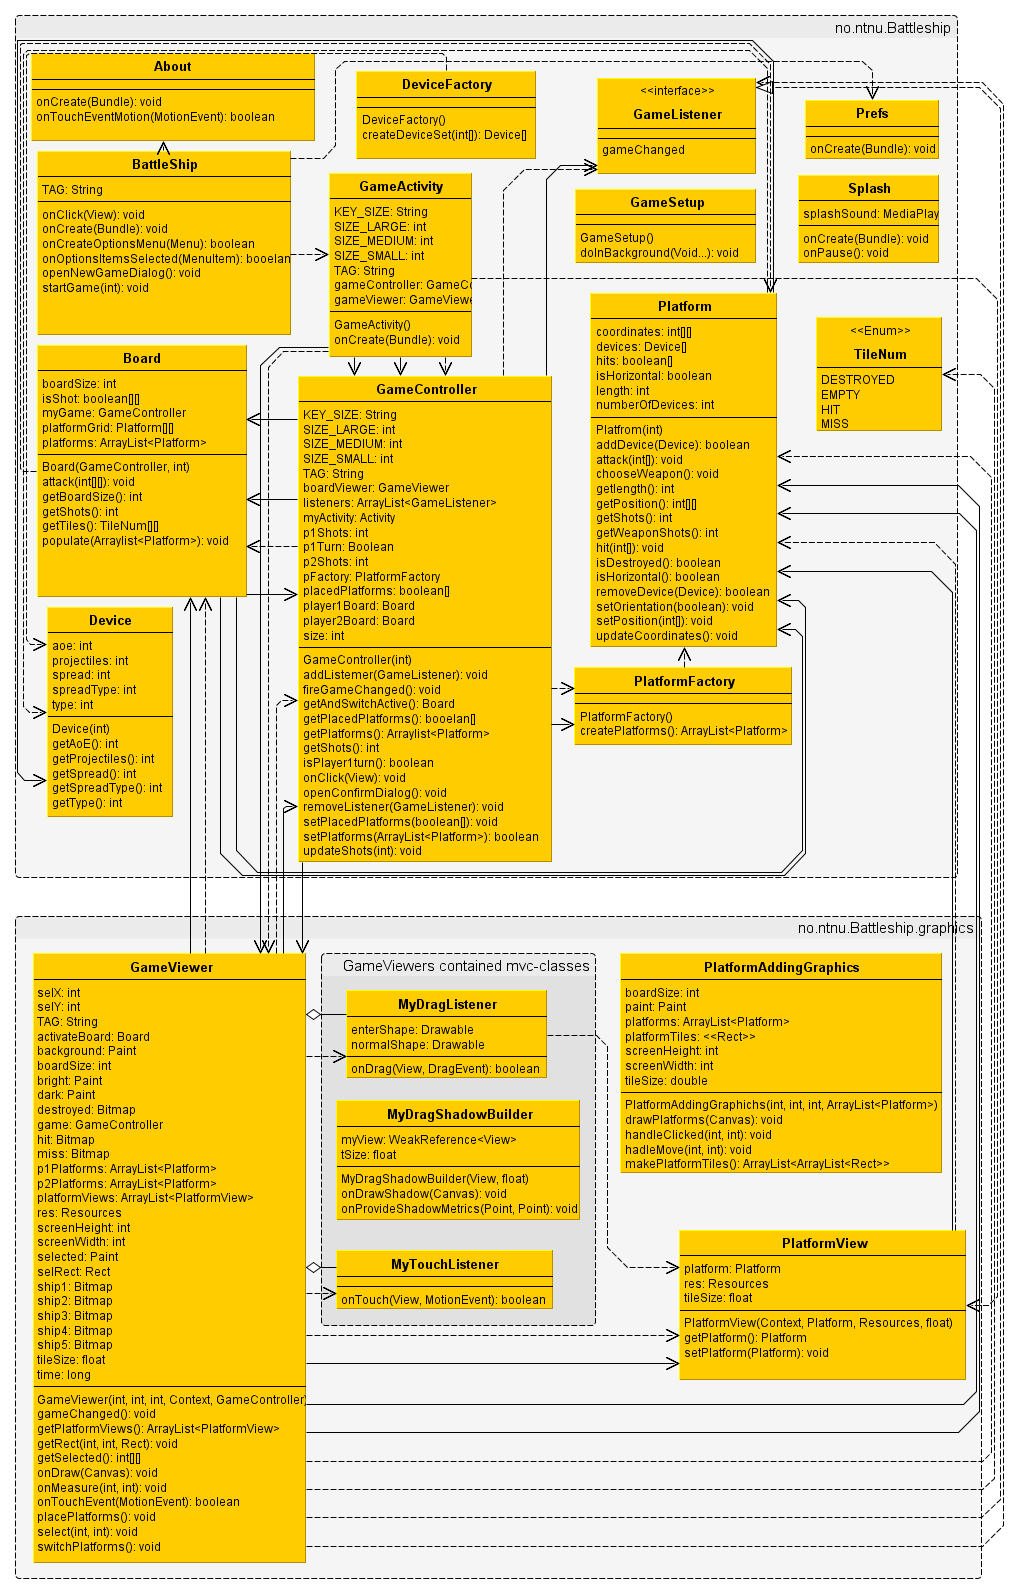
\includegraphics[width=\textwidth]{classdiagram} 
    \caption{The class diagram}
    \label{fig:classdiagram}
\end{figure}

\section{Test reports:}
\subsection{Funtional requirements}
\paragraph{FR0:} Player shall be able to place platforms with devices\\
\begin{tabular}{  p{.3\textwidth}  p{.7\textwidth} }
	Executor: & Håkon Hesselberg  \\
	Date: & 24.04.2013 \\
	Time: & 10:59 - 11:04  \\
	Evaluation: & Sccess \\
	Comment: & After starting a new game and selecting a10x10 board it was
possible to drag and drop the platforms. \\
\end{tabular}

\paragraph{FR1:} Player shall be able to click \\
\begin{tabular}{  p{.3\textwidth}  p{.7\textwidth} }
    Executor: & Håkon Hesselberg  \\
    Date: & 24.04.2013 \\
    Time: & 11:04 - 11:05  \\
    Evaluation: & Sccess \\
    Comment: & \\
\end{tabular}

\paragraph{FR2:} Player shall be able to click platforms\\
\begin{tabular}{  p{.3\textwidth}  p{.7\textwidth} }
    Executor: & Håkon Hesselberg  \\
    Date: & 24.04.2013 \\
    Time: & 11:05 - 11:07  \\
    Evaluation: & Sccess \\
    Comment: & Clicking on a platform as of now does nothing, but
double-clicking flips the ship between horizontal and vertical, and this works \\ 
\end{tabular}

\paragraph{FR3:} Player shall be able to click empty squares\\
\begin{tabular}{  p{.3\textwidth}  p{.7\textwidth} }
    Executor: & Håkon Hesselberg  \\
    Date: & 24.04.2013 \\
    Time: & 11:07 – 11:11 \\
    Evaluation: & Sccess \\
    Comment: & Clicking on a blue (empty) square after the game as started and
the ships have been placed turns the square green, indicating that it has been
clicked\\
\end{tabular}

\paragraph{FR4:} Player shall be able to win\\
\begin{tabular}{  p{.3\textwidth}  p{.7\textwidth} }
    Executor: & Bremnes, Jan A. S. \\
    Date: & 25.04.2013 \\
    Time: & 11:38 - 11:45  \\
    Evaluation: & Sccess \\
	Comments: & Upon destroying every enemy ship the player is greeted with a
win-message\\
\end{tabular}

\paragraph{FR5:}  Player shall be able to lose\\
\begin{tabular}{  p{.3\textwidth}  p{.7\textwidth} }
    Executor: & Bremnes, Jan A. S. \\
    Date: & 25.04.2013 \\
    Time: & 11:38 - 11:45  \\
    Evaluation: & Sccess \\
    Comment: & 
As there is only local multiplayer, when a player has won it means that the
other player has lost \\
\end{tabular}

\paragraph{FR6:} System shall support local multiplayer\\
\begin{tabular}{  p{.3\textwidth}  p{.7\textwidth} }
    Executor: & Håkon Hesselberg  \\
    Date: & 24.04.2013 \\
    Time: & 11:12 - 11:12  \\
    Evaluation: & Sccess \\
	Comment: &

\end{tabular}

\paragraph{FR7:} System shall play sounds\\
\begin{tabular}{  p{.3\textwidth}  p{.7\textwidth} }
    Executor: & Håkon Hesselberg  \\
    Date: & 24.04.2013 \\
    Time: & 11:21 - 11:22  \\
    Evaluation: & Sccess \\
	Comment: &
A sound is displayed upon startup while the splash screen is shown\\
\end{tabular}

\paragraph{FR8:} Player shall be able to place platforms with devices\\
\begin{tabular}{  p{.3\textwidth}  p{.7\textwidth} }
    Executor: & Håkon Hesselberg  \\
    Date: & 24.04.2013 \\
    Time: & 11:23 - 11:25  \\
    Evaluation: & Sccess \\
	Comment: &
Works on several different emulated devices \\
\end{tabular}

\subsection{Quality requirements:}
\paragraph{QR0:} The application shall not crash more than once every 1000
moves\\
\begin{tabular}{  p{.3\textwidth}  p{.7\textwidth} }
    Executor: & Everyone \\
    Date: & 22.04.2013 - 24.04.2013 \\
    Time: & Varied \\
    Stimuli: & Performing moves \\
    Expected response: & The game gets played normally without crashing \\
    Observed response: & All testing done over several days have yet to result in a crash \\
    Evaluation: & Success \\
    Comment: & This was a test done in bits every time someone on the group did something with \\
the app \\
\end{tabular}

\paragraph{QR1:} The application shall register clicks at least 75\% of the time
\\
\begin{tabular}{  p{.3\textwidth}  p{.7\textwidth} }
	Executor: & Everyone \\
	Date: & 22.04.2013 - 24.04.2013 \\
	Time: & Varied \\
	Stimuli: & Performing actions\\
    Expected response: & Clicks get registered, causing the app to do the correct action. \\
    Observed response: & Most of the time everything went as expected \\
    Evaluation: & Success \\
    Comment: & This was a test done in bits every time someone on the group did something with \\
\end{tabular}

\paragraph{QR2:} The application shall correctly calculate the correct result of an
action at least 99.9\% of the time \\
\begin{tabular}{  p{.3\textwidth}  p{.7\textwidth} }
    Executor: & Everyone \\
    Date: & 22.04.2013 - 24.04.2013 \\
    Time: & Varied \\
    Stimuli: & Performing actions \\
    Expected response: & The correct action is performed \\
    Observed response: & The correct action does not get performed correctly 99.9\% of the time \\
    Evaluation: & Failure \\
    Comment: & More bug-fixing is needed \\
\end{tabular}

\paragraph{QR3:} The application shall scale and run correctly on at least 75\% of
tested devices running the tested version of android\\
\begin{tabular}{  p{.3\textwidth}  p{.7\textwidth} }
    Executor: & Håkon Hesselberg \\
    Date: & 24.04.2013 \\
    Time: & 11: & 46 – 12: & 15 \\
    Stimuli: & Starting a game on several different devices \\
    Expected response: & The game scales correctly and runs \\
    Observed response: & It worked on every device \\
    Evaluation: & Success \\
    Comment: & Five different emulated devices were used \\
\end{tabular}

\paragraph{QR4:} The game shall recognize the correct player as the winner at
least 99\% of the time \\
\begin{tabular}{  p{.3\textwidth}  p{.7\textwidth} }
    Executor: & Bremnes, Jan A. S. \\
    Date: & 25.04.2013 \\
    Time: & 11: & 38-11: & 45 \\
    Stimuli: & Playing the game until a winner is declared \\
    Expected response: & The correct player is shown as the winner \\
    Observed response: & 100\% of the time the correct player was recognized as the winner \\
    Evaluation: & Success \\
    Comment: &  \\
\end{tabular}

\paragraph{QR5:} MTBF shall be at least 1 hour\\
\begin{tabular}{  p{.3\textwidth}  p{.7\textwidth} }
    Executor: & Everyone \\
    Date: & 22.04.2013 – 25.04.2013 \\
    Time: & Varied \\
    Stimuli: & Leaving emulator open with game running, performing actions once in  while \\
    Expected response: & Game works as intended and does not crash \\
    Observed response: & Application did not crash \\
    Evaluation: & Success \\
    Comment: &  \\
\end{tabular}

\paragraph{QR6:} The application shall not brick any of the developers' phones
or computers \\
\begin{tabular}{  p{.3\textwidth}  p{.7\textwidth} }
    Executor: & Everyone \\
    Date: & Entire project \\
    Time: & Varied \\
    Stimuli: &  \\
    Expected response: & No bricking \\
    Observed response: & It worked \\
    Evaluation: & Success \\
    Comment: &  \\
\end{tabular}

\section{Architecture Relationship}
\paragraph{MVC:}\\
MVC has turned out to have no implementation standard among existing apps, some
developers going so far as to theorize that google has intentionally made it
hard to implement to discourage its use. We’ve had to do extensive refactoring
during the implementation phase to keep it as MVC compatible as possible, and we
feel that we’ve been able to pull it off fairly well. There are however still a
few places in the code where MVC has not been strictly implemented, most notably
in the use of a button listener in the GameController class. We attribute this
partly to the difficulty of MVC on android, but primarily to time constraints
during the last implementation sprint.
The difficulties surrounding MVC on android are not all that well documented,
and it would have been hard to spot earlier in the project than we did, but the
time constraints we could have discovered them earlier by using extensive time
estimation, but at the time we felt it would consume more time than we would
have gained.

\paragraph{Abstract factories:}\\
As of final delivery, only the skeleton and base functionalities of these have
been implemented.
The plan was to have the factories interconnect and use external configuration
files to provide multiple game modes. What has been implemented is the platform
factory, with a single hardcoded game mode, and no device support.
We however feel that modifying the skeleton device factory, and the platform
factory wouldn’t require any modification of the rest of the codebase, and as
such we’ve succeeded in providing a solid base architecture to work off of and
their full implementation would be a mere matter of man hours.

\section{Issues}
We should have made a more detailed plan based on the architecture before
starting working on it. As an example, we should clearly have defined what
classes we desired to use for graphics, what methods they should have, and what
they should do, not just stating that “we need graphics”.
We should also have communicated more within the group about specifics. For an
instance, when one part of the group set out to do graphics, did graphics, and
then later another part of the group changed those graphics.
As for what we could’ve done better we could have planned for and used a third
party package with a simple and well documented API for doing all the graphics. 

\section{Future work}
	There is still a lot of work that remains to be done in order to make the game we originally planned. In its current state the game is nothing more than any other Battleship game, while we originally intended to make an expanded version. We had planned on letting players choose different kind of weapons platforms, instead of just ships, and let them choose which devices to place on these platforms, all of which would have different properties. Due to a severe underestimate of the difficulties involved in writing the game for Android, this was never implemented. Classes are in place for the implementation of different platforms and devices, so it should be relatively easy to implement at some point in the future. The ability to save the current game state and resume playing an old game, and the addition of background music is also something that could be done. Of more advanced functionality, we can mention support for network multiplayer.


\section{Time spent}
\begin{tabular}{  p{.3\textwidth} p{.2\textwidth} p{.5\textwidth} }
    Name & Hours &  Duty \\
    Bremnes, Jan A. S. & 100  & Programming, testing, report writing.\\
    Johanessen, Stig Tore & 100 & Architectural patterns and report.\\
    Hesselberg, Håkon H. & 100 & Testing, report writing, programming.\\
    Kirø, Magnus L. & 100 & Architecture input, system design and report writing.\\
    Randby, Simon G. & 100 & Report writing, documentation, programming.\\
    Tørresen, Håvard & 100 & Programming, testing, report writing.\\
\end{tabular}

\section{Discussion}
TODO

\end{document}
